\documentclass[border=2mm,12pt,tikz]{standalone}
\usepackage{tikz-3dplot} 
\usepackage{bm}
\usetikzlibrary{intersections,patterns.meta}
\begin{document}
    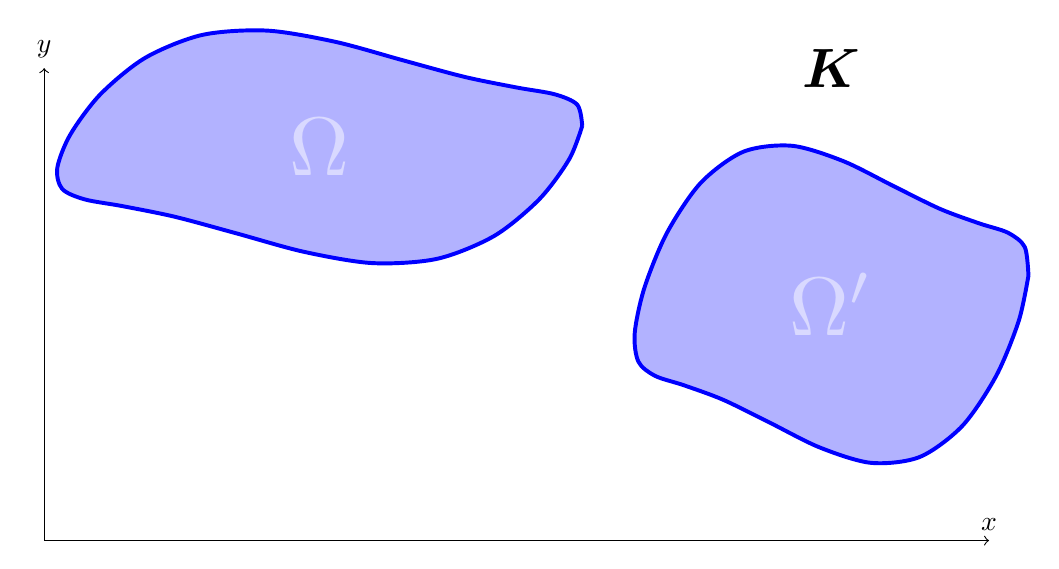
\begin{tikzpicture}[
        mdomain/.style = {blue, line width = 0.5mm, fill = blue, fill opacity = 0.3}
    ]
        \draw[mdomain] plot[smooth, variable=\u, domain=0:360]({(5 * cos(\u) + 0.3 * sin(\u))/1.5 + 3.5},{(2 * sin(\u) + 0.4 * cos(3 *\u))/1.5+5});
        \draw[mdomain] plot[smooth, variable=\u, domain=0:360, blue, thick, fill = blue, fill opacity = 0.6]({(5 * cos(\u) + 0.3 * sin(\u))/2 +10},{(2 * sin(\u) + 0.4 * cos(3 *\u))/1.1+3});

        \node[white, scale = 3, opacity = 0.5] (A) at (3.5,5) {$\Omega$};
        \node[white, scale = 3, opacity = 0.5] (B) at (10,3) {$\Omega'$};
        \node[scale = 2] at (10,6) {$\bm{K}$};


        \draw[->] (0,0) -- (12,0) node[above]{$x$};
        \draw[->] (0,0) -- (0,6) node[above]{$y$};

                
        
    \end{tikzpicture}
\end{document} 